\chapter{Design measurements}
\label{cha:measurements}
For measuring the effect of different designs on the simulations performance a example network was implemented using a monolithic and a modular design.
These implementations represent examples of the designs discussed in chapter \ref{cha:design}.


\section{Simulated example network}
\label{sec:measurements_network}
The example network simulates a message queue with dispatching of different types of transmitted data (configuration, event, historical).
The different types of data are processed by different parts within the network.
This network includes parts for data generation and data processing.
Such a exemplary network was chosen, due to multiple similar practical applications.
An overview of the simulated network is shown in Figure \ref{fig:design_test_network}.

\begin{figure}
    \centering
    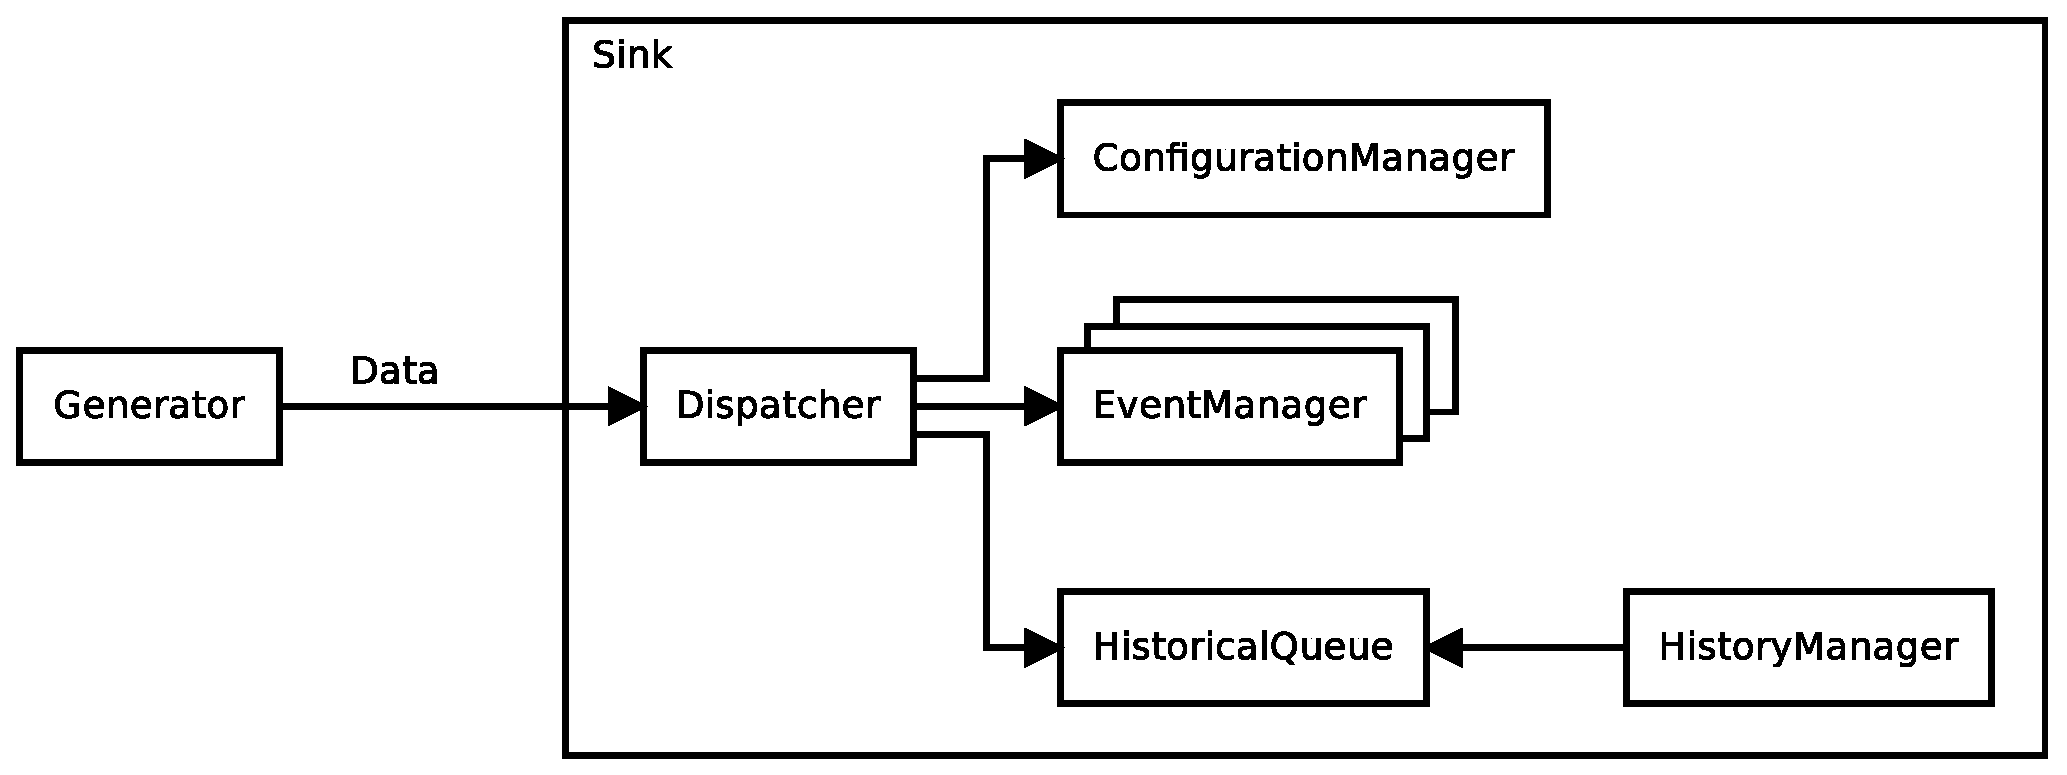
\includegraphics[width=0.9\linewidth]{design_test_network.eps}
    \caption{Example network including \emph{Generator}, \emph{Sink}, \emph{HistoricalQueue} and the data processing modles \emph{ConfigurationManager}, \emph{EventManager}, and \emph{HistoryManager}.}
    \label{fig:design_test_network}
\end{figure}

The \emph{Generator} generates cyclic data which are transmitted via messages to the sink module.
The generated data includes a field of 64 Bytes and a enumeration describing the type of data.

These messages are transmitted to a sink, which is described via the interface module \emph{ISink}.
The differently designed modules \emph{ModularSink} and \emph{MonolithicSink} extend the interface and represent the different tested designs.

The first part within the sink is the \emph{Dispatcher} which is accessing the type information of the data and then forwards the packed data to the according managers or the \emph{HistoricalQueue}.
The simulated network provides a variable number of \emph{EventManagers}, all generated event data are dispatched to the \emph{EventManagers} sequentially.
The \emph{ConfigurationManager} and the \emph{EventManagers} are simple implementations which executes various calculations on the received data to simulate processing.
Historical data are forwarded to the \emph{HistoricalQueue} which is internally implemented by a std::queue which holds all received data until they are accessed.
The \emph{HistoryManager} accesses the \emph{HistoricalQueue} and processes available data similar to \emph{ConfigurationManager} and \emph{EventManager} by executing dummy calculations.
This access is initiated by the \emph{HistoryManager} itself and provides a configurable polling interval.
\\

The functionality of dispatching and processing the data is, as shown in Figure \ref{fig:design_test_network}, included in the sink and is implemented twice with different designs.

The assumption of existing implementations for the \emph{Dispatcher}, \emph{HistoricalQueue}, \emph{ConfigurationManager}, \emph{EventManager} and \emph{HistoryManager} is made.
This assumption should connect this design test to practical scenarios where existing code cannot be changed for the simulation.
Therefore implementing the \emph{MonolithicSink} consists of instantiating and connecting the different parts within a single simple module.
Received messages will be analyzed and the enclosed data is forwarded to the according instances.
The polling is done by the \emph{ConfigurationManager} using \emph{self-messages} sent in an configurable interval.

Implementing the \emph{ModularSink} requires the implementation of wrapper modules for every single part which should be represented by a separate module.
These wrapper extract the transmitted data of received messages and forward it to the enclosed parts.
Calls from within the enclosed parts are handled by methods of the wrappers, which are passed via function pointers (functional objects).
Within this methods according messages are created and sent via the correct output gates.
The internal structure of the \emph{ModularSink} is shown in figure \ref{fig:ModularSink}.
Within the \emph{ModularSink} arrays of gates, connections and instances of \emph{EventWrappers} are used for realizing a variable number of \emph{EventManagers}.

\begin{figure}
    \centering
    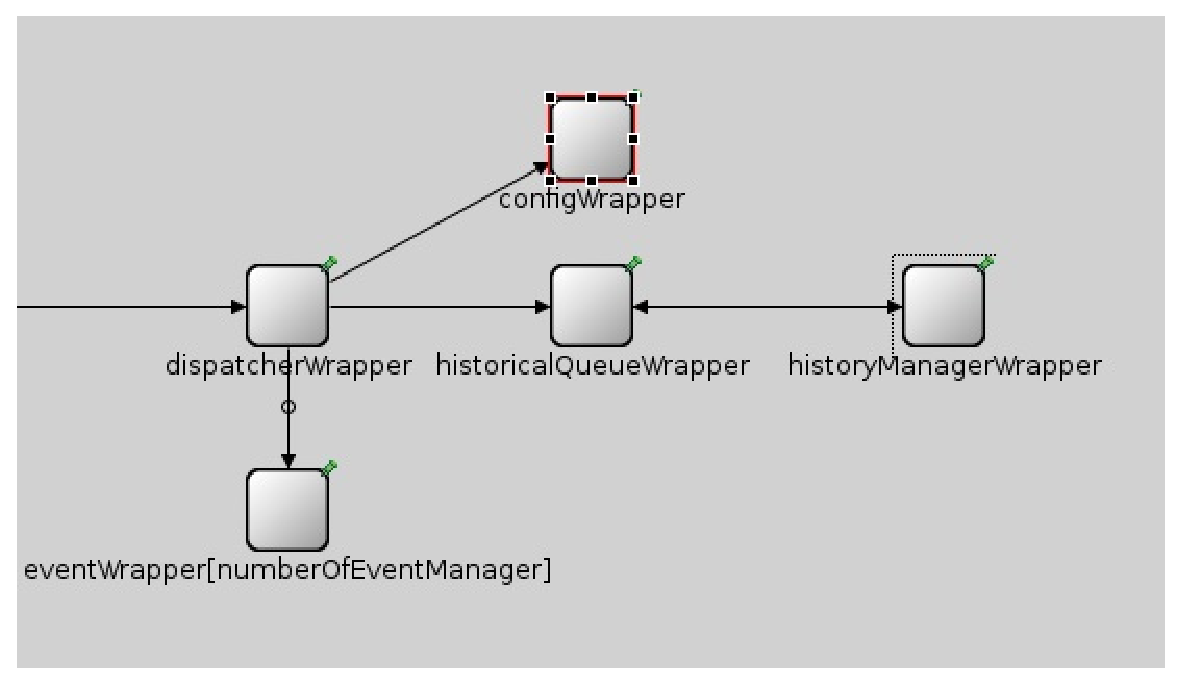
\includegraphics[width=0.9\linewidth]{images/ModularSink}
    \caption{Structure of \emph{ModularSink} showing the implemented wrapper modules and their connections.}
    \label{fig:ModularSink}
\end{figure}

The simulated network consists of the \emph{Generator} instance and a instance specializing \emph{ISink} the underlying module and therefore the tested design is configured via a variable type.
The resulting network for data generation is shown in figure \ref{fig:omnet_example_network}.

\begin{figure}
    \centering
    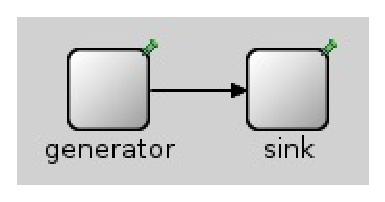
\includegraphics[width=0.3\linewidth]{images/omnet_example_network}
    \caption{Simulated example network showing the \emph{Generator} instance and its connection to the instance of the sink module derived from \emph{ISink}.}
    \label{fig:omnet_example_network}
\end{figure}

\section{Measurement methods}
\label{sec:measurements_methods}
For measuring the performance of the different designs three measurement methods were implemented
Three different methods were implemented for preventing false assumptions based on the result of a single test.
These methods were implemented via different scripts for automated executing and designed dynamically allowing the analyze of various simulations and also either sequential or parallel simulation.

\subsection{Runtime measurement}
\label{sec:measurements_methods_runtime}
The performance of the simulated design can be analyzed by defining a fixed simulation time limit (\emph{sim-time-limit}).
Using the default (non real-time) scheduler this results in a simulation which executes as fast as possible for the required number of events for reaching the simulation time limit.
The required execution time for this simulation represents the performance of the simulation.

Analyzing a parallel simulation using this method does not require special attention, except the handling of multiple resulting runtime values.

\subsection{Processed event count}
\label{sec:measurements_methods_event}
By defining a fixed execution time limit (\emph{cpu-time-limit}) and using the default scheduler the simulation will run for a fixed time.
The number of processed events within this fixed time represents the performance of the simulation.

The simulation of different designs results in contrasting event counts due to the varying number of messages using other designs with more modules and therefore more communication.
For comparison of the performance the created number within a fixed processing time a correction factor must be considered.
This factor describes the ratio of create events using the different designs.
This ratio can be measured using the configuration of the previous method \ref{sec:measurements_methods_runtime} and analyzing the number of created events.

Analyzing a parallel simulation and comparing the performance to a sequential simulation requires further attention to the number of created events.
An additional correction factor is necessary due to the varying number of sent synchronization messages.

\subsection{Real time behavior}
\label{sec:measurements_methods_realtime}
Using the built in real time scheduler \emph{cRealTimeScheduler} the simulation will try to execute the simulation matching the real time.
The performance output (\emph{cmdenv-performance-display}) provides the ratio of simulated seconds per real second.
As described in section \ref{sec:simulation_omnet} this ratio must not differ too much from one for representing a real-time simulation.
The simulated network provides a configurable interval of data generation by \emph{Generator}.
Using a parameter study (described in section \ref{sec:omnet_running_config}) the interval for data generation by \emph{Generator} can be set to values form a range of intervals.
With attention to the performance ratio of the different iterations the interval limit, which still allows real-time simulation, can be determined.

\subsection{Result recording}
The results of the different measurement methods are all extracted from the resulting command line output of the simulation.
The automated test scripts are analyzing the outputs of the executed simulation after finishing the simulation.
For preventing the delay of the measurements and the simulation by writing the output to a file located on an slow peripheral the output files are located on a \emph{ramdisk}.
A \emph{ramdisk} represents a filesystem which is located within the \emph{RAM} (Random access memory) and therefore provides the maximum speed for writing and analyzing outputs.

The implemented test network described in \ref{sec:measurements_network} was developed and analyzed on a Lenovo ideapad U530 with 8GB PC3-12800 DDR3 SDRAM 1600 MHz and a 4th Gen Intel® Core™ i7-4500U (1.8 GHz 200 MHz 4MB) running Kubuntu 15.10.
\cite{lenovo_spec}

\section{Sequential Simulation}
\label{sec:measurements_sequential}
Each of the three developed measurement methods was executed multiple times with the example network.
To eliminate a possible dependency of the resulting performance to the simulated range (e.g. period of simulation time) each method was executed with different times.
The runtime and real-time method was executed for multiple values for the simulation time limit and the event method was executed for different cpu time limits.
This variation of simulation time verifies the testing measurements for independence of the simulated time range and provides reference values for determining correction values for the event method \ref{sec:measurements_methods_event}.

Simulating multiple scenarios three parameter studies (parameter sweeps) were executed for each testing method.

\begin{itemize}
    \item Number of EventManager (default = 1)
    \item Generation interval of \emph{Generator} (default = $100\mu s$)
    \item Polling interval of \emph{HistoryManager} (default = $100\mu s$)
\end{itemize}

During the simulation with different values of a single parameter study the other values are set to the default values.
For the testing scenarios the simulation time limit for the runtime and real-time method or the cpu time limit for the event method was set to one minute.
In the following section the measurement result of the evaluation test (sweep of simulation or cpu time) and the results of the test scenarios are shown and analyzed.

\subsection{Runtime}
\label{sec:measurements_sequential_runtime}

The runtime results of the sequential simulations using both designs and given different simulation time limits are displayed in figure \ref{fig:results_runtime_sim_time}.
The double logarithmic axis shows two linear characteristics for modular and monolithic design.
These nearly parallel linear characteristics show a constant factor in between the runtimes using the two different designs.
The average ratio of runtime using the modular design over the runtime using the monolithic design is $3.393$. %TODO refresh
\\

%TODO check if necessary
% \[\frac{\sum\frac{t_{modular}}{t_{monolithic}}}{N} = 2.84\]

%%% runtime over simulation time %%%
\begin{figure}
    \centering
    \pgfplotsset{
        every axis plot/.append style={very thick}
    }
    \begin{tikzpicture}
        \begin{axis}[
        xmode=log,
        ymode=log,
        ylabel={Runtime $[s]$},
        xlabel={Simulation time $[s]$},
        grid=major,
        legend entries={Modular,Monolithic},
        legend style={at={(0.03,0.97)}, anchor=north west}
        ]
        
        \addplot table {results/runtimeResults.Modular.txt};
        \addplot table {results/runtimeResults.Monolithic.txt};
        \end{axis}
    \end{tikzpicture}    
    \caption{Runtime using different designs over different simulation time limits.}
    \label{fig:results_runtime_sim_time}
\end{figure}

The runtime using different designs with a varying number of \emph{EventManagers} is shown in figure \ref{fig:results_runtime_eventmanager}.
As expected there is no obvious dependency of the resulting runtime to the number of included \emph{EventManagers}.
Due to the fixed simulation time the number of created event stays the same.
The only difference introduced by the increasing number of \emph{EventManagers} is the destination of the event typed data.
The required time for transporting the messages and processing the data is untouched.
The increasing number affects the memory usage of the simulation, which is not analyzed within this design test.
The offset, visible in figure \ref{fig:results_runtime_eventmanager}, in between the different designs is representing the ratio of achieved performance regarding the runtime.
The average of this ratio is $3.342$.
\\

%%% runtime over number of event manager %%%
\begin{figure}
    \centering
    \pgfplotsset{
        every axis plot/.append style={very thick}
    }
    \begin{tikzpicture}
    \begin{axis}[
    xmode=log,
    %ymode=log,
    ylabel={Runtime [s]},
    xlabel={Number of \emph{EventManager}},
    grid=major,
    legend entries={Modular,Monolithic},
    legend style={at={(0.97,0.5)},anchor=east}
    ]
    
    \addplot table {results/time/simtimeEventManagerResults.Modular.txt};
    \addplot table {results/time/simtimeEventManagerResults.Monolithic.txt};
    \end{axis}
    \end{tikzpicture}    
    \caption{Runtime using different designs over variing number of \emph{EventManager}.}
    \label{fig:results_runtime_eventmanager}
\end{figure}

The runtime using different designs with a varying polling interval by the \emph{HistoryManager} is shown in figure \ref{fig:results_runtime_polling}.
These results are again shown in a double logarithmic plot for easier recognition of both plots following a potential characteristic, which is visible as linear plots.
As expected the required runtime is sinking with increasing polling interval.
This behavior can be explained by the sinking frequency of polling operations and thus a decreasing communication.
The offset in between the two plots shown in figure \ref{fig:results_runtime_polling} is, due to the double logarithmic display, representing the ratio in between the runtimes using different designs.
The average ratio of runtime using the modular design over the runtime using the monolithic design is $7.809$.
\\
%%% runtime over polling interval %%%
\begin{figure}
    \centering
    \pgfplotsset{
        every axis plot/.append style={very thick}
    }
    \begin{tikzpicture}
    \begin{axis}[
    xmode=log,
    ymode=log,
    ylabel={Runtime [s]},
    xlabel={Polling interval [ns]},
    grid=major,
    legend entries={Modular,Monolithic},
    legend style={at={(0.97,0.97)}, anchor=north east}
    ]
    
    \addplot table {results/time/simtimePollingResults.Modular.txt};
    \addplot table {results/time/simtimePollingResults.Monolithic.txt};
    \end{axis}
    \end{tikzpicture}    
    \caption{Runtime using different designs over varying polling interval by the \emph{HistoryManager}.}
    \label{fig:results_runtime_polling}
\end{figure}

The runtime using different designs with a varying generation interval by the \emph{Generator} is shown in figure \ref{fig:results_runtime_generation}.
Similar to the previous figure these results are also shown in a double logarithmic plot showing the potential characteristic of sinking required runtime with increasing generation interval.
Again the noticeable offset in between the plots is due to a ratio of resulting runtimes.
The average ratio of runtime using the modular design over the runtime using the monolithic design is $1.588$.
\\

%%% runtime over generation interval %%%
\begin{figure}
    \centering
    \pgfplotsset{
        every axis plot/.append style={very thick}
    }
    \begin{tikzpicture}
    \begin{axis}[
    xmode=log,
    ymode=log,
    ylabel={Runtime [s]},
    xlabel={Generation interval [ns]},
    grid=major,
    legend entries={Modular,Monolithic},
    legend style={at={(0.97,0.97)}, anchor=north east}
    ]
    
    \addplot table {results/time/simtimeGenerationResults.Modular.txt};
    \addplot table {results/time/simtimeGenerationResults.Monolithic.txt};
    \end{axis}
    \end{tikzpicture}    
    \caption{Runtime using different designs over varying generation interval by the \emph{Generator}.}
    \label{fig:results_runtime_generation}
\end{figure}


Analyzing the resulting outputs the ratio of generated messages (events) regarding the different designs can be determined.
The average ratio of number of created events using the modular design over the number of created events using the monolithic design is $2.149$.
This ratio will be used as correction value for the next measurement method analyzing the created events within a fixed cpu time.

\subsection{Created events}
\label{sec:measurements_sequential_event}

The results of testing the simulations and analyzing the number of created events within a given cpu time are displayed in figure \ref{fig:results_event_cpu_time}.
Similar to the previous section a double logarithmic display was used for analyzing the characteristic of the plots.
The courses show potential characteristics and are nearly linear and parallel this leads to the assumption of a constant ratio in between the used designs.
The average ratio of number of created events using the modular design over the number of created event using the monolithic design is $0.284$. %TODO refresh
For comparison to the previous and following test method the reciprocal value is calculated and equals $3.521$.
\\

%TODO check if necessary
%\[\frac{\sum\frac{eventcount_{modular}}{eventcount_{monolithic}}}{N} = 0.549\]

%%% event number over cpu time %%%
\begin{figure}
    \centering
    \pgfplotsset{
        every axis plot/.append style={very thick}
    }
    \begin{tikzpicture}
        \begin{axis}[
        xmode=log,
        ymode=log,
        ylabel={Created event},
        xlabel={Cpu time $[s]$},
        grid=major,
        legend entries={Modular,Monolithic},
        legend style={at={(0.03,0.97)}, anchor=north west}
        ]
        
        \addplot table {results/eventResults.Modular.txt};
        \addplot table {results/eventResults.Monolithic.txt};
        \end{axis}
    \end{tikzpicture}    
    \caption{Created events for different designs over different cpu time limits.}
    \label{fig:results_event_cpu_time}
\end{figure}

The number of created events using different designs and a varying number of \emph{EventManagers} is showed in figure \ref{fig:results_event_eventmanager}.
As expected and similar to the results of the runtime with a varying number of \emph{EventManagers} there is no noticeable dependency of the created events to the number of \emph{EventManagers}.
This presumption was done because by changing the number of instantiated \emph{EventManagers} only the destination of the transmitted events is affected but not the number of events.
Using the double logarithmic visible as offset the ratio in between the different designs is showed in figure \ref{fig:results_event_eventmanager}.
This ratio is defined by the number of created events using a modular design over the number of created events using a monolithic design.
The average of this ratio is $0.273$.
For comparison to the previous and following test method the reciprocal value is calculated which equals $3.663$.
\\

%%% events over Event managers %%%
\begin{figure}
    \centering
    \pgfplotsset{
        every axis plot/.append style={very thick}
    }
    \begin{tikzpicture}
    \begin{axis}[
    xmode=log,
    %ymode=log,
    ylabel={Created events},
    xlabel={Number of EventManager},
    grid=major,
    legend entries={Modular,Monolithic},
    legend style={at={(0.97,0.5)},anchor=east}
    ]
    
    \addplot table {results/event/cputimeEventManagerResults.Modular.txt};
    \addplot table {results/event/cputimeEventManagerResults.Monolithic.txt};
    \end{axis}
    \end{tikzpicture}    
    \caption{Created events using different designs over varying number of \emph{EventManager}.}
    \label{fig:results_event_eventmanager}
\end{figure}

The number of created events using different designs and a varying polling interval by the \emph{HistoryManager} is shown in figure \ref{fig:results_event_polling}.
This result is leading to the assumption of no definable dependency of the number of created events to the polling interval of \emph{HistoryManager}.
The offset in between the plots using different designs is although indicating a ratio representing the performance difference of the used designs.
This ratio is defined by the number of created events using a modular design over the number of created events using a monolithic design.
The average of this ratio results for this test in $0.166$.
For comparison to the previous and following test method the reciprocal value is calculated and equals $6.024$.
\\

%%% events over polling interval %%%
\begin{figure}
    \centering
    \pgfplotsset{
        every axis plot/.append style={very thick}
    }
    \begin{tikzpicture}
    \begin{axis}[
    xmode=log,
    ymode=log,
    ylabel={Created events},
    xlabel={Polling interval [ns]},
    grid=major,
    legend entries={Modular,Monolithic},
    legend style={at={(0.97,0.5)},anchor=east}
    ]
    
    \addplot table {results/event/cputimePollingResults.Modular.txt};
    \addplot table {results/event/cputimePollingResults.Monolithic.txt};
    \end{axis}
    \end{tikzpicture}    
    \caption{Created events using different designs over variing polling interval by the \emph{HistoryManager}.}
    \label{fig:results_event_polling}
\end{figure}

The number of created events using different designs and a varying generation interval by the \emph{Generator} is shown in figure \ref{fig:results_event_generation}.
Similar to the polling interval of \emph{HistoryManager} shown in \ref{fig:results_event_polling} there is no dependency identifiable.
The offset is related to the ratio in between the designs and the average ratio is $0.436$.
For comparison to the previous and following test method the reciprocal value is calculated and equals $2.294$.
\\

%%% events over generation interval %%%
\begin{figure}
    \centering
    \pgfplotsset{
        every axis plot/.append style={very thick}
    }
    \begin{tikzpicture}
    \begin{axis}[
    xmode=log,
    ymode=log,
    ylabel={Created events},
    xlabel={Generation interval [ns]},
    grid=major,
    legend entries={Modular,Monolithic},
    legend style={at={(0.97,0.5)},anchor=east}
    ]
    
    \addplot table {results/event/cputimeGenerationResults.Modular.txt};
    \addplot table {results/event/cputimeGenerationResults.Monolithic.txt};
    \end{axis}
    \end{tikzpicture}    
    \caption{Created events using different designs over variing generation interval by the \emph{Generator}.}
    \label{fig:results_event_generation}
\end{figure}

\subsection{Real-time}
\label{sec:measurements_sequential_realtime}

The real-time results of the sequential simulations using both designs and given different simulation time limits are displayed in figure \ref{fig:results_realtime_sim_time}.
The simulation time limit defines the runtime of a real-time simulation, but does not affect the performance, i.e. the frequency and complexity of calculations.
Therefore the result shows as expected no recognizable dependency of the achievable generation interval to the simulation time.
Although an offset in between the different designs is visible.
This offset represents the ratio of achievable generation interval using a modular design over the achievable generation interval using a monolithic design.
The average of this ratio is $1.717$.\\

% realtime over sim time
\begin{figure}
    \centering
    \pgfplotsset{
        every axis plot/.append style={very thick}
    }
    \begin{tikzpicture}
        \begin{axis}[
        xmode=log,
        ymode=log,
        ylabel={Achievable real time generation interval [ns]},
        xlabel={Simulation time [s]},
        grid=major,
        legend entries={Modular,Monolithic},
        legend style={at={(0.97,0.97)}, anchor=north east}
        ]
        
        \addplot table {results/realTimeResults.Modular.txt};
        \addplot table {results/realTimeResults.Monolithic.txt};
        \end{axis}
    \end{tikzpicture}    
    \caption{Real-time results for different designs over different simulation time limits.}
    \label{fig:results_realtime_sim_time}
\end{figure}

The real-time results for a varying number of \emph{EventManagers} is shown in figure \ref{fig:results_realtime_eventmanager}.
The resulting characteristics show a wide distribution and therefore does not lead to a clear assumption about a to the number of \emph{EventManagers}.
The impact of the different designs is still noticeable.
The average ratio of the achievable generation interval using different designs is $1.488$.
\\

% realtime over event managers
\begin{figure}
    \centering
    \pgfplotsset{
        every axis plot/.append style={very thick}
    }
    \begin{tikzpicture}
    \begin{axis}[
    xmode=log,
    ymode=log,
    ylabel={Achievable real time generation interval [ns]},
    xlabel={Number of \emph{Eventmanagers}},
    grid=major,
    legend entries={Modular,Monolithic},
    legend style={at={(0.97,0.5)}, anchor=east}
    ]
    
    \addplot table {results/realtime/rtEventManagerResults.Modular.txt};
    \addplot table {results/realtime/rtEventManagerResults.Monolithic.txt};
    \end{axis}
    \end{tikzpicture}    
    \caption{Real-time results for different designs over a varying number of \emph{EventManagers}.}
    \label{fig:results_realtime_eventmanager}
\end{figure}

The real-time results for a varying polling interval of \emph{HistoryManager} is shown in figure \ref{fig:results_realtime_polling}.
Similar to the previous results there is no noticeable dependency of the achievable generation interval to the used polling interval.
The performance difference is again shown in the ratio of the achieved intervals.
The average of this ratio is $99999$.
%TODO add average
\\

% realtime over polling interval
\begin{figure}
    \centering
    \pgfplotsset{
        every axis plot/.append style={very thick}
    }
    \begin{tikzpicture}
    \begin{axis}[
    xmode=log,
    ymode=log,
    ylabel={Achievable real time generation interval [ns]},
    xlabel={Polling interval of \emph{HistoryManager} [ns]},
    grid=major,
    legend entries={Modular,Monolithic},
    legend style={at={(0.97,0.5)}, anchor=east}
    ]
    
    \addplot table {results/realtime/rtPollingResults.Modular.txt};
    \addplot table {results/realtime/rtPollingResults.Monolithic.txt};
    \end{axis}
    \end{tikzpicture}    
    \caption{Real-time results for different designs over a varying polling interval of \emph{HistoryManager}.}
    \label{fig:results_realtime_polling}
\end{figure}

The measurement method for analyzing the real-time behavior includes a parameter study of the generation interval of the \emph{Generator}.
Therefore the scenario with varying generation intervals cannot be analyzed using the real-time method.

\subsection{Conclusion of sequential design tests}
\label{sec:measurements_sequential_conclusion}

The analyzed methods were also executed on two additional host machines:

\begin{description}
    \item[Workstation] including an Intel  running Windows 7.
    \item[Build Server] running Linux Mint 17. %TODO????
\end{description}}

Analyzing the results displayed in section \ref{sec:measurements_sequential_runtime}, \ref{sec:measurements_methods_event} and \ref{sec:measurements_methods_realtime} the following insights were made:

\begin{itemize}
    \item Using a modular design the number of events created is bigger, for example the simulated test network resulted in a ratio of created events for a modular design over a monolithic of $9999$. %TODO insert event avg
    \item The increased number of events and the included overhead results in an decreased performance noticeable in each of the three used measurement methods.
    \item The average performance ratio analyzing the runtime is $9999$. %TODO insert runtime avg
    \item The average performance ratio analyzing the real time behavior is $9999$. %TODO insert realtime avg
    \item Varying load simulated by decreased polling interval or generation interval shows a bigger impact on the performance of the modular design network.
\end{itemize}

Using the sequential simulation a monolithic design is recommended for real-time simulations.


\section{Parallel simulation}
\label{sec:measurements_parallel}
The parallel simulation was executed using the \emph{MPI} system openMPI for communication.
The used synchronization method was the \emph{Null Message Protocol} described in section \ref{sec:parallel_omnet_sync}.
A explicit synchronization of the different partitions is necessary due to multiple modules which are using \emph{self-messages} as timers.
The host machine used for developing and executing the simulation provides a 4th Gen Intel® Core™ i7-4500U (1.8 GHz 200 MHz 4MB).
This processor is a dual core CPU supporting hyper threading and therefore provides four logical processors distributed on two physical cores.
The example network includes two autonomous modules which are scheduling their behavior with \emph{self-messages}.
This number of autonomous modules leads to the conclusion for two parallel partitions for parallel simulation.

As described in chapter \ref{cha:parallel_sim} running a simulation distributed on parallel devices requires the mapping of the simulated modules to different parallel partitions.
The first mapping can be applied to both designs and assigns the \emph{Generator} to the partition zero and all modules within the \emph{Sink} to the partition one.
The second tested mapping assigns all modules to the partition zero excepting the \emph{HistoryManager}, which is assigned to the partition one.

As the ratio in between the number of created events by a modular or a monolithic design, described in section \ref{sec:measurements_methods_event}, running a parallel simulation also requires a correction factor due to the varying number of created events by different partitioning.
This dependency is caused by the changing set of transmitted data messages and required synchronization messages.

This correction value can also be determined using the previously discussed method \ref{sec:measurements_methods_runtime}.
The impact of synchronization within parallel simulations is described in section \ref{sec:parallel_omnet_sync}.

\subsection{Runtime}
\label{sec:measurements_parallel_runtime}


\subsection{Event}
\label{sec:measurements_parallel_event}


\subsection{Real-time}
\label{sec:measurements_parallel_realtime}

\subsection{Conclusion of parallel tests}

Considering the results shown in the sections \ref{sec:measurements_parallel_runtime}, \ref{sec:measurements_parallel_event} and \ref{sec:measurements_parallel_realtime} the following insights were made:

\begin{itemize}
    \item The performance of a parallel simulation is depending strongly on the simulated model and its partitioning capabilities.
    \item The used synchronization is highly affecting the achievable performance.
\end{itemize}

\section{Conclusion}
Considering the results of section \ref{sec:measurements_sequential} and \ref{sec:measurements_parallel} the modular design is mostly resulting in a increased number of messages and the caused overhead leads to a debased performance.
Analyzing the simulation of the chosen example network the parallel simulation was not able to achieve an improved performance in comparison to the sequential simulation.
The capabilities of parallel simulation, especially for the usage in the fields of real-time simulation, emulation and \emph{HiL} must be analyzed individually for each simulated model. 